\documentclass[12pt,epsf,psfig,graphics]{article}             
\textwidth = 6.5in
\textheight = 9.05in
\topmargin 0.0in
\oddsidemargin 0.0in
\evensidemargin 0.0in

% set it so that subsubsections have numbers and they
% are displayed in the TOC (maybe hard to read, might want to disable)

\usepackage[T1]{fontenc}
\usepackage{mathptmx}

\usepackage{graphics}
\usepackage{pifont}
\setcounter{secnumdepth}{3}
\setcounter{tocdepth}{3}

% define widow protection 
        
\def\widow#1{\vskip #1\vbadness10000\penalty-200\vskip-#1}

% define a little section heading that doesn't go with any number

\def\littlesection#1{
\widow{2cm}
\vskip 0.5cm
\noindent{\bf #1}
\vskip 0.1cm
\noindent
}

% A paraphrase mode that makes it easy to see the stuff that shouldn't
% stay in for the final proposal

\newdimen\tmpdim
\long\def\paraphrase#1{{\parskip=0pt\hfil\break
\tmpdim=\hsize\advance\tmpdim by -15pt\noindent%
\hbox to \hsize
{\vrule\hskip 3pt\vrule\hfil\hbox to \tmpdim{\vbox{\hsize=\tmpdim
\def\par{\leavevmode\endgraf}
\obeyspaces \obeylines 
\let\par=\endgraf
\bf #1}}}}}

\renewcommand{\baselinestretch}{1.2}    % must go before the begin of doc
\newtheorem{principle}{Principle}
\newtheorem{definition}{Definition}
\newtheorem{define}{Definition}
% go with the way that CC sets the margins

\usepackage{listings}

\usepackage{color}

\definecolor{javared}{rgb}{0.6,0,0} % for strings
\definecolor{javagreen}{rgb}{0.25,0.5,0.35} % comments
\definecolor{javapurple}{rgb}{0.5,0,0.35} % keywords
\definecolor{javadocblue}{rgb}{0.25,0.35,0.75} % javadoc

\newcommand*\yes{\item[\Checkmark]}
\newcommand*\yesplus{\item[\Checkmark$^{+}$]}
\newcommand*\yesminus{\item[\Checkmark$^{-}$]}

\newcommand*\no{\item[\small{\XSolidBrush}]}

\begin{document}

\lstset{language=Java,
basicstyle=\ttfamily,
keywordstyle=\color{javapurple}\bfseries,
stringstyle=\color{javared},
commentstyle=\color{javagreen},
morecomment=[s][\color{javadocblue}]{/**}{*/},
%numbers=left,
numberstyle=\scriptsize\color{black},
stepnumber=1,
numbersep=7pt,
tabsize=4,
showspaces=false,
showstringspaces=false}

% handle widows appropriately
\def\widow#1{\vskip #1\vbadness10000\penalty-200\vskip-#1}

\begin{center}

CMPSC 440: Operating Systems\\
Final Examination \\
%Saturday December 11, 2004 \\

\end{center}

\noindent Answer the ten questions that are listed on the following pages.  You must provide answers to these questions
on a separate sheet of paper.  Please develop responses that clearly express your ideas in the most succinct manner
possible.  You are not permitted to complete this examination in conjunction with any of your classmates.  Furthermore,
you cannot consult any outside references during this examination.  If you have questions concerning the following
problems, then please visit my office during the examination period.  If you leave the classroom to take the exam, then
you are responsible for checking the white board for status updates.

%\mbox{} \newline
%\mbox{} \newline

\begin{enumerate}

\item ({\bf 10 Points}) The process is the main ``unit of work'' in an operating system.  Answer the following questions
  about processes and how they are managed by the operating system.

  \begin{enumerate}

    \item ({\bf 5 Points}) In order to manage the execution of a process, an operating system must contain a wide
      variety of software components and leverage different types of hardware.  Draw a complete diagram of an operating
      system that graphically depicts:

      \begin{enumerate}

        \item The operating system kernel
        \item The existence of user programs
        \item The hardware of a modern computer
        \item The interface between the hardware and the software
        \item The interaction between kernel and user programs

      \end{enumerate}

    \item ({\bf 3 Points}) A process can be in one of three states: running, blocked, and ready. Using circles to
      represent each of these states and directed edges to denote transitions between these states, draw a process-state
      diagram. All states and edges must have labels.

    \item ({\bf 2 Points}) The operating system maintains a process table that stores information about each process
      that is currently executing on a computer. Using concrete examples whenever possible, please name and describe at
      least two of these fields.

  \end{enumerate}

  \newpage

\begin{figure}[t]
  \centering
  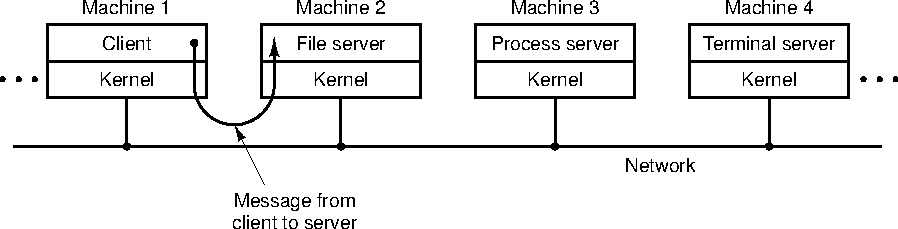
\includegraphics{fig1-27}
  \caption{Client-Server Communication Involving the Client, a Server, and the Kernel.}
  \label{fig:clientserver}
\end{figure}

\item ({\bf 10 Points}) There are many basic concepts that undergird the fundamentals of operating systems.  Answer the
  following questions about basic operating systems concepts.

  \begin{enumerate}
          
  \item ({\bf 4 Points}) A real-time operating system must schedule tasks to guarantee that a specified deadline will be
    met.  Draw a graph with a horizontal axis called ``time'', a vertical axis called ``utility'', and a vertical line
    at point $D$ on the horizontal axis.  Now, please draw a utility curve that represents the challenge associated with
    scheduling in a real-time operating system. Why did you draw this curve the way that you did?

  \item ({\bf 3 Points}) The shell of an operating system allows for the composition of processes using the pipe and
    filter architecture.  In the following code segment, what is the pipe? What is the filter? Why is this a good mode
    of interaction with the operating system?

    \begin{quote}
      {\tt cat file1 file2 file3 | sort > /dev/lp \&}
    \end{quote}

  \item ({\bf 3 Points}) Figure~\ref{fig:clientserver} furnishes an example of client-server communication with the
    support of the operating system kernel. Please outline all of the steps that must take place to support the
    communication between ``Machine 1'' and ``Machine 2''. 

  \end{enumerate}

  \newpage

\item ({\bf 10 Points}) The memory management unit (MMU) of an operating system controls what parts of a program are in
  memory and how those programs parts are accessed.  Answer the following questions about basic memory management
  operations and their trade-offs.
  
  \begin{enumerate}

    \item ({\bf 3 Points}) Many computers have both RAM and ROM.  What is the meaning of these two terms?  How does a
      computer operating system use both RAM and ROM? Does the computer store the Basic Input/Output System (BIOS) in
      the RAM or the ROM?

    \item ({\bf 4 Points}) It is possible to divide up the computer's memory into address spaces.  What is an address
      space?  What does it mean if an address space is dynamically relocatable? How could the MMU use the base and limit
      registers to support dynamic relocation?   

    \item ({\bf 3 Points}) The majority of modern operating systems support both virtual and physical memory.  After
      clearly defining both of these types of memory, please state which one is faster and explain why this is the case.
      Why does an OS support both of these?

  \end{enumerate}
        
\newpage

% \begin{figure}[t]
%   \centering
%   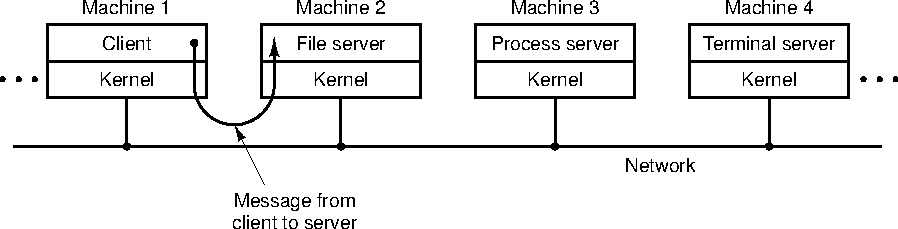
\includegraphics{fig1-27}
%   \caption{Client-Server Communication Involving the Client, a Server, and the Kernel.}
%   \label{fig:clientserver}
% \end{figure}
% 
\item ({\bf 10 Points}) It is important for the memory management unit (MMU) to be able to track the memory that is
  currently free.  Answer the following questions about managing free memory.

  \begin{enumerate}
          
  \item ({\bf 4 Points}) Suppose that the memory manager keeps a linked list of allocated and free segments.  Next,
    assume that the MMU tracks the following information for each unit of the memory; in this notation $P$
    denotes ``Process'' and $H$ stands \mbox{for ``Hole''}.

    \begin{itemize}
      \item The type marker, $T \in \{P, H\}$
      \item The start location, $S$
      \item The length of the unit, $L$
    \end{itemize}

    Using the aforementioned information that is tracked for each allocation unit, please clearly explain how the
    following memory allocation algorithms would work.

    \begin{enumerate}
      \item ({\bf 2 Points}) First fit
      \item ({\bf 2 Points}) Best fit
      % \item ({\bf 2 Points}) Worst fit
      % \item ({\bf 2 Points}) Quick fit
    \end{enumerate}

  \item ({\bf 3 Points}) The memory manager should use an efficient algorithm to allocate a program to a free location in
    memory.  What is the worst-case time complexity of the first fit and best fit algorithms?  Which, if any, of these
    two algorithms is likely to be faster?

  \item ({\bf 3 Points}) Peter J.\ Denning proposed the working set model to characterize a program's use of computer
    memory.  Draw a graph that visualizes the standard understanding of the working set.  Your graph should contain the
    following entities:

    \begin{enumerate}

      \item A vertical axis with the label $w(k, t)$
      \item A horizontal axis with the label $k$
      \item A curve that shows the relationship between $w(k, t)$ and $k$

    \end{enumerate}

  You may assume the following meanings for the notation in the diagram:

  \begin{enumerate}

    \item $t$ is the current time in the operating system
    \item $k$ denotes the number of the most recent memory references
    \item$w(k, t)$ is the size of the working set at time $t$ for the past $k$ references  

  \end{enumerate}

  \end{enumerate}

  \newpage

\item ({\bf 10 Points}) An operating system's memory manager often segments the memory into pages.  Answer the following
  questions about memory pages and page replacement algorithms.

  \begin{enumerate}

    \item ({\bf 2 Points}) What is a page fault? What does an operating system do when one occurs?

    \item ({\bf 2 Points}) The optimal page replacement algorithm is the ``gold standard'' by which other page
      replacement algorithms are judged.  How does this algorithm work? 

    \item ({\bf 4 Points}) Page replacement algorithms can use two bits to determine which page should be replaced.
      These bits, $R$ and $M$, have the following meanings:

      \begin{itemize} 
        \item $R$: the page was referenced 
        \item $M$: the page was modified
      \end{itemize}
  
    The not recently used (NRU) algorithm removes a page at random from the lowest-numbered non-empty class, with the
    four classes having the following names:

    \begin{itemize}
      \item Class 0
      \item Class 1
      \item Class 2
      \item Class 3
    \end{itemize}
    
    Using the $R$ and $M$ bits in your response, what is the meaning of these four classes?

    \item ({\bf 2 Points}) One of the aforementioned classes contains an entity known at the VIP.  What is the meaning
      of this term? What does the NRU algorithm do with these VIPs?

  \end{enumerate}

  \newpage
  
\item ({\bf 10 Points}) An operating system normally provides a file system that supports the persistent storage of
  data.  Answer the following questions about the creation and use of file systems.

  \begin{enumerate}

    % \item ({\bf 4 Points}) Operating systems commonly support both sequential-access and random-access files.  What is
    %   the meaning of these two terms?  What type of file would a database management system use to store its contents?
    %   Why?

    \item ({\bf 4 Points}) File system traversal involves the automated visitation of all of the files and directories
      in a specified region of the file system. Using either Java source code or pseudo code, implement a complete file
      system traversal method.

    \item ({\bf 4 Points}) A file system often supports navigation of directories with both relative and absolute path
      names.  What is the meaning of these two terms?  Please give an example of each path type and explain what
      indicates that the path is either relative or absolute.

    \item ({\bf 2 Points})  The following line is excerpted from an {\tt /etc/fstab} file on a Linux workstation.  What
      is the meaning of these two lines? At minimum, your response to this question should clearly explain the meaning
      of the terms {\tt /dev/sda1} and {\tt ext4}. \\

      \hspace*{-.75in}
      \vspace*{1in}
      \begin{minipage}{4in}
        \begin{verbatim}
        # / was on /dev/sda1 during installation
        UUID=5f006f4b-ff6c-4d12-9e78-a3540f33339e / ext4 errors=remount -ro 0 1
        \end{verbatim}
      \end{minipage}

  \end{enumerate}

  \newpage

  % \begin{figure}[p]
  %   \centering
  %   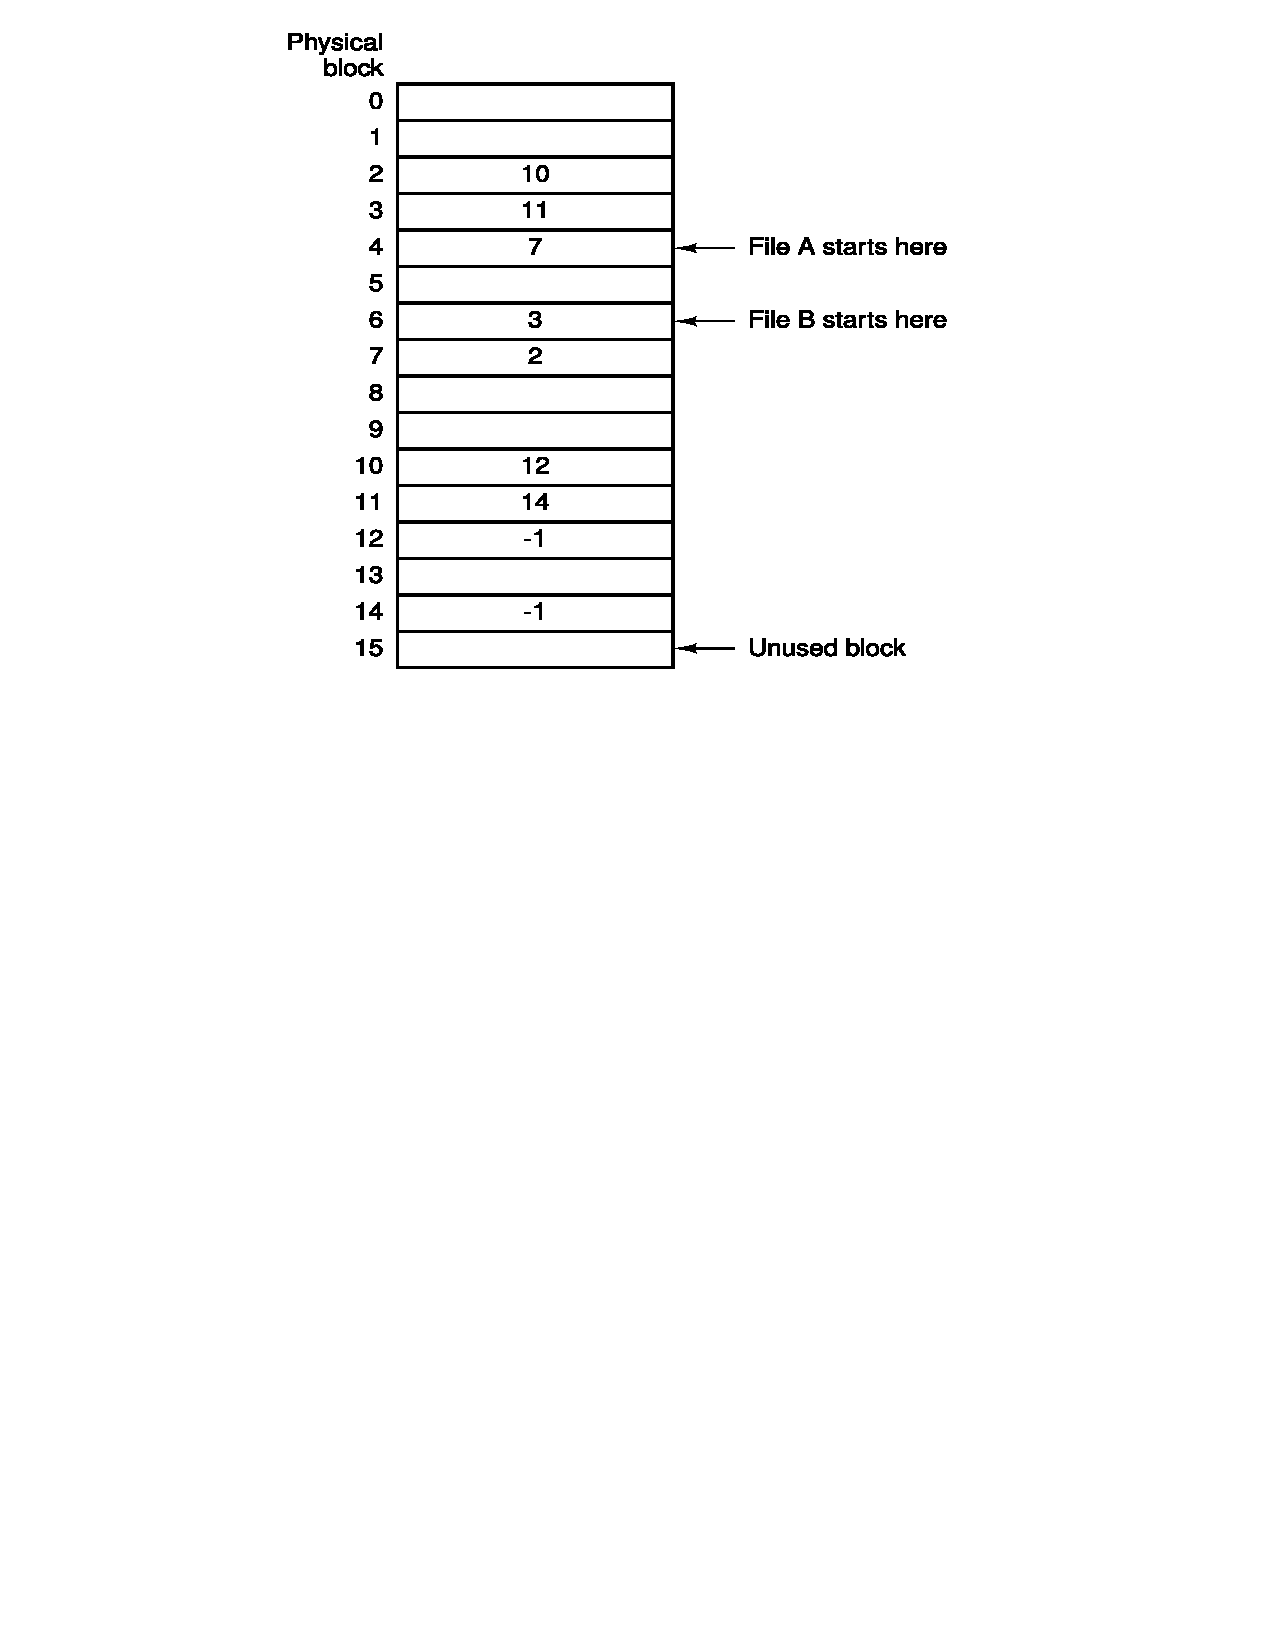
\includegraphics{fig412}
  %   \vspace*{-6.75in}
  %   \caption{A Structure for File Management.}
  %   \label{fig:fat}
  % \end{figure}

% \item ({\bf 10 Points}) The file system must have an efficient implementation of files and directories that supports
%   rapid creation, deletion, and location.  Answer the following questions about file system implementation and
%   the use of disk drives.
% 
% \begin{enumerate}
% 
%   \item ({\bf 5 Points}) Figure~\ref{fig:fat} shows one example of a structure that a file system can use to manage
%     files.  What is the name of this structure? How does a file system use this structure to find files?  What are the
%     drawbacks associated with this approach?
% 
%   \item ({\bf 3 Points}) Certain file systems, such as NTFS, provide support for journaling.  What is a
%     journaling file system?  What are the benefits and drawbacks associated with journals?
% 
%   \item ({\bf 2 Points}) It is possible to have a file system run on a solid-state drive (SSD).  What is an SSD?  What
%     are the benefits associated with the use of SSDs? 
% 
% \end{enumerate}
% 
% \newpage

\item ({\bf 10 Points}) Computer hardware contains a wide variety of input/output devices that the operating system must
  manage.  Answer the following questions about these devices.

  \begin{enumerate}

    \item ({\bf 4 Points}) A computer system can contain both volatile and non-volatile memory.  What are the
      similarities and differences between these two types of memory?  Please give a situation in which it would be
      advisable to use each type of memory.

    \item ({\bf 3 Points}) Many operating systems, like GNU/Linux, support the X Windows System.  What role do the X
      client, X server, and the X protocol have in running an interface?

    \item ({\bf 3 Points}) The main paradigm for computing often oscillates between the use of thin clients and fat
      clients.  What is the meaning of these two terms?  After furnishing an appropriate definition of these client
      types, please give an example of a situation in which one of the types would be best according to a well-defined
      metric.

  \end{enumerate}

  \newpage

\item ({\bf 10 Points}) Given the high cost of electricity and batteries, it is important for an operating system to
  support power management.  Answer the following questions about this topic.

  \begin{enumerate}

    \item ({\bf 4 Points}) Why would it be useful to run a power management module in the operating system that runs on
      either a server or a mobile device? Your response to this question should furnish two reasons for the server and
      two for the mobile device.

    \item ({\bf 4 Points}) There are many different components of a computation device such as a laptop or a
      tablet.  What are three of the most ``power hungry'' parts of these devices? 

    \item ({\bf 2 Points}) Suppose that you are implementing an operating system's power-management module for the
      central processing unit (CPU).  What are two strategies that you could implement to reduce the CPU's consumption
      of power?

  \end{enumerate}

  \newpage

\item ({\bf 10 Points}) An operating system for a multi-processor device often contains algorithms for deadlock
  detection and avoidance.  Answer the following questions about deadlocks.

  \begin{enumerate}

    \item ({\bf 4 Points}) Coffman et al.\ showed that there are four conditions that must hold for there to be a
      resource deadlock. What are these four conditions?

    \item ({\bf 4 Points}) It is possible to model the use of resources in a multi-processor operating system with a
      resource allocation graph (RAG).  What is the meaning of the nodes and the edges in a RAG?  How does the structure
      of the RAG indicate that the operating system is in deadlock? Your response to this question should furnish a
      graphical depiction of a RAG that shows the evidence of a system in deadlock.

    \item ({\bf 2 Points}) The ostrich algorithm is one method for managing deadlocks in an operating system.  How does
      the ostrich algorithm work? What are the benefits of this approach?

  \end{enumerate}

  \newpage

\item ({\bf 10 Points}) Operating systems also play a major role in the deployment and use of distributed systems.
  Answer the following questions about distributed systems.

  \begin{enumerate}

    \item ({\bf 4 Points}) Most distributed systems employ a middleware.  What is middleware?

    \item ({\bf 6 Points}) The JavaSpace is an example of a middleware that supports loosely-coupled communication.
      After describing the three main operations supported by a JavaSpace, your response to this question should explain
      why the JavaSpace supports loosely-coupled communication. What are the efficiency and effectiveness trade-offs
      associated with the use of a JavaSpace? Please use a diagram to support all of your points.

  \end{enumerate}

\end{enumerate}

\end{document}

